\documentclass[root.tex]{subfiles}

\begin{document}
	
	{\pagestyle{empty}}
	\section{Showcase Maneuver}
	\label{chap:Showcase_Maneuver}
	To briefly show the general functioning and to give the reader insight into a practical application of the project, a standard driving maneuver was performed on the platform in the outlined \gls{HIL} configuration. As an example the U-turn was chosen, for its relevance in everyday driving and the fact that it shows some of the characteristics of \glspl{LCV} distinctively. It was executed at a longitudinal speed of 2\unit{m/s}, thus resulting in a turning radius of approx. 16\unit{m}. To ensure consistent behaviour over all measurements, the steering-angles of the truck were pre-programmed. As visible from figure \ref{fig:Path}, the truck does not leave the turn in a perfectly straight path. However this is not really relevant to this verification, as discussed further on only matching between the two environments is called for.
	
	\begin{figure}[!h]
		
		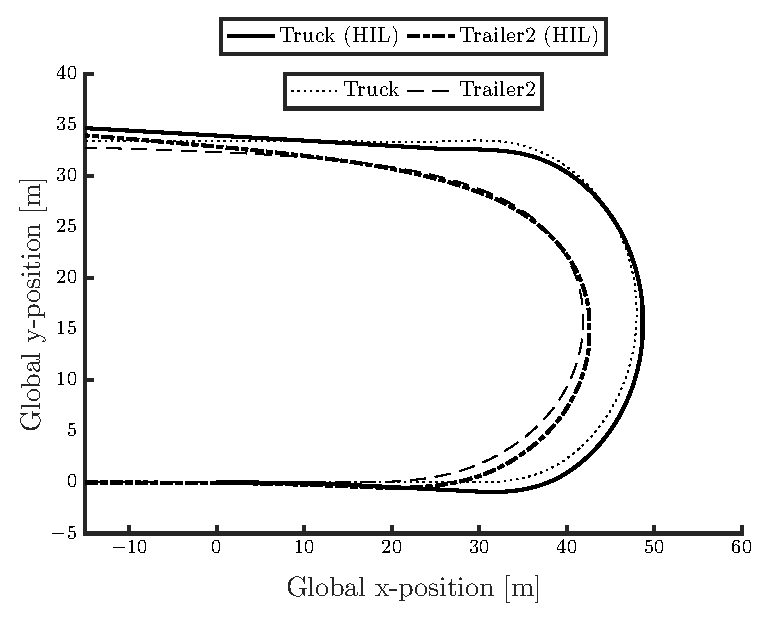
\includegraphics[width=0.9\linewidth]{xy_HIL_and_VTM}
		\caption[Path of Tractor and Second Trailer for HiL and Simulation]{Path of Tractor and Second Trailer for HiL and Simulation}
		
		\label{fig:Path}
	\end{figure}
	
	
	Figure \ref{fig:Path} shows the behaviour of the different units of the combination both for the developed platform in its \gls{HIL}-configuration as well as the performance in the simulation environment. This gives the opportunity to compare between the two different stages of abstraction in the V-model, thus verifying the correct functioning of the actuated axles before executing further testing in the V-model:
	
	It clearly shows in figure \ref{fig:Path} is the phenomenon, that the second trailer does not follow  the tractors path exactly. This is called off-tracking and minimizing it with an adequate actuation strategy is one of the major points within this research project. However this shall only be a brief mention in this publication. 
	
	The main point of figure \ref{fig:Path} however is, to show the congruence of the resulting trajectories of the simulated environment and the \gls{HIL}-setup. 
	
	
	
	
		
	

	
\end{document}